\chapter{Curves}
\label{chapter:curves}
%Begin Section 1.8
\section{Vector-Valued Functions}
Now that we are familiar with vectors and their operations, we can begin discussing functions whose values are
vectors.\index{function!vector-valued}

\statedefn{defn:vecfcn}{
{A \textbf{vector-valued function of a real variable} is a rule that associates a vector $\mathbf{f}(t)$ with a real
number $t$, where $t$ is in $\Real{}$ or its interval (called the \textbf{domain} of $\mathbf{f}$). 
We write
$\mathbf{f}: D \rightarrow \Real{3}$ to denote that $\mathbf{f}$ is a mapping of $D$ into $\Real{3}$.}
}

For example, $\mathbf{f}(t) = t \mathbf{i} + t^2 \mathbf{j} + t^3 \mathbf{k}$ is a vector-valued function in $\Real{3}$,
defined for all real numbers $t$. 
We would write $\mathbf{f}: \Real{} \rightarrow \Real{3}$. 
At $t = 1$
the value of the function is the vector $\mathbf{i} + \mathbf{j} + \mathbf{k}$, which in Cartesian coordinates has the
terminal point $(1,1,1)$.

A vector-valued function of a real variable can be written in component form as
\begin{displaymath}
 \mathbf{f}(t) = \ssub{f}{1}(t) \mathbf{i} + \ssub{f}{2}(t) \mathbf{j} + \ssub{f}{3}(t) \mathbf{k}\quad\text{or}\quad\mathbf{f}(t) = ( \ssub{f}{1}(t),\ssub{f}{2}(t),\ssub{f}{3}(t) )
\end{displaymath}
for some real-valued functions $\ssub{f}{1}(t)$, $\ssub{f}{2}(t)$, $\ssub{f}{3}(t)$, called the \emph{component 
functions} of $\mathbf{f}$. 
The first form is often used when emphasizing that $\mathbf{f}(t)$ is a vector, and the second form is useful when considering just the terminal points of the vectors.

\smallskip
\hrule width \textwidth height 0.5pt
\piccaption[]{}\parpic[r]{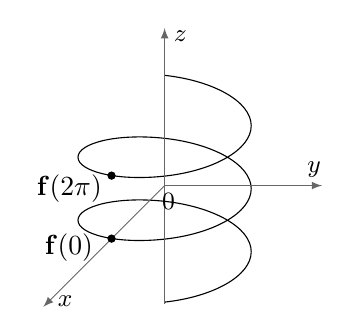
\begin{tikzpicture}
 \usetikzlibrary{arrows}
 \usetikzlibrary{snakes}
 \definecolor{spherecolor}{HTML}{80DCFF}
 \definecolor{planecolor}{HTML}{FFB270}
 \draw [rotate=-90][snake=coil,segment amplitude=1.1cm,segment length=.8cm,segment aspect=0.4] (-1.4,0) -- (1.5,0);
 \draw [black!60,line width=0.3pt,-latex] (0,0) -- (2,0,0);
 \draw [black!60,line width=0.3pt,-latex] (0,-1.5) -- (0,2,0);
 \draw [black!60,line width=0.3pt,-latex] (0,0) -- (0,0,4);
 \pgfputat{\pgfpointxyz{1.9}{0.2}{0}}{\pgfbox[center,center]{\small $y$}};
 \pgfputat{\pgfpointxyz{0.2}{1.9}{0}}{\pgfbox[center,center]{\small $z$}};
 \pgfputat{\pgfpointxyz{0.2}{0}{3.8}}{\pgfbox[center,center]{\small $x$}};
 \pgfputat{\pgfpointxyz{0.05}{-0.2}{0}}{\pgfbox[center,center]{\small $0$}};
 \fill (0,0,1.75) circle (1.5pt);
 \node [below,left] at (-0.1,-0.1,1.78) {$\mathbf{f}(0)$};
 \fill (0,0.8,1.75) circle (1.5pt);
 \node [below,left] at (0,0.64,1.75) {$\mathbf{f}(2 \pi)$};
\end{tikzpicture}
}
\begin{exmp}
 Define $\mathbf{f}: \mathbb{R} \rightarrow \Real{3}$ by $\mathbf{f}(t) = ( \cos t , \sin t , t )$.\\ 
 This is a parametric equation of a \emph{helix}\index{helix} (see Figure 1.8.1). 
 As the value of $t$ increases, the terminal points of
 $\mathbf{f}(t)$ is spiraling upward. 
 For each $t$, the $x$- and $y$-coordinates of $\mathbf{f}(t)$
 are $x = \cos t$ and $y = \sin t$, so
 \begin{displaymath}
 x^2 + y^2 = \cos^2 t + \sin^2 t = 1.
 \end{displaymath}
 Thus, $\mathbf{f}(t)$ lies on the surface of the right circular cylinder $x^2 + y^2 = 1$ for any $t$.
\end{exmp}
\hrule width \textwidth height 0.5pt
\smallskip

Since each of the three component functions are real-valued, it will sometimes be the case that results
from single-variable calculus can simply be applied to each of the component functions to yield a similar result for the
vector-valued function. However, there are times when such generalizations do not hold (see Exercise 13). The concept of
a limit, though, can be extended naturally to vector-valued functions, as in the following definition.

\statedefn{defn:veclim}{
 {Let $\mathbf{f}(t)$ be a vector-valued function, let $a$ be a real number and let $\mathbf{c}$ be a vector. Then we say
 that the \textbf{limit}\index{limit!vector-valued function} of $\mathbf{f}(t)$ as $t$ approaches $a$ equals $\mathbf{c}$,
 written as
  $\lim\limits_{t \to a} \mathbf{f}(t) = \mathbf{c}$,
 if $\lim\limits_{t \to a} \,\norm{\mathbf{f}(t) - \mathbf{c}} = 0$. 
 
 Equivalently, if
 $\mathbf{f}(t) = ( \ssub{f}{1}(t),\ssub{f}{2}(t),\ssub{f}{3}(t) )$, then
 \begin{displaymath}
  \lim_{t \to a} \mathbf{f}(t) =
  \biggl( \lim_{t \to a} \ssub{f}{1}(t), \lim_{t \to a} \ssub{f}{2}(t), \lim_{t \to a} \ssub{f}{3}(t) \biggr),
 \end{displaymath}
 provided that all three limits on the right side exist.}
}

The above definition shows that continuity and the derivative of vector-valued functions can also be
defined in terms of its component functions.\index{continuity}\index{derivative!vector-valued function}
\statedefn{defn:veccont}{
 {Let $\mathbf{f}(t) = ( \ssub{f}{1}(t),\ssub{f}{2}(t),\ssub{f}{3}(t) )$ be a vector-valued function, and let $a$ be a
 real number in its domain. Then $\mathbf{f}(t)$ is \textbf{continuous} at $a$ if
 $\lim\limits_{t \to a} \mathbf{f}(t) = \mathbf{f}(a)$. Equivalently, $\mathbf{f}(t)$ is continuous at $a$ if and only
 if $\ssub{f}{1}(t)$, $\ssub{f}{2}(t)$, and $\ssub{f}{3}(t)$ are continuous at $a$.\\
 The \textbf{derivative} of $\mathbf{f}(t)$ at $a$, denoted by $\mathbf{f}'(a)$ or $\dfrac{d \mathbf{f}}{dt}(a)$,
 is the limit
 \begin{displaymath}
  \mathbf{f}'(a) = \lim_{h \to 0} \frac{\mathbf{f}(a + h) - \mathbf{f}(a)}{h}
 \end{displaymath}
 }
 \par\noindent if that limit exists. Equivalently, $\mathbf{f}'(a) = ( \ssub{f}{1}'(a),\ssub{f}{2}'(a),
 \ssub{f}{3}'(a) )$, if the component derivatives exist. We say that $\mathbf{f}(t)$ is \textbf{differentiable} at
 $a$ if $\mathbf{f}'(a)$ exists.
}

A real-valued function whose first derivative is continuous is called\index{arc length}
\emph{continuously differentiable}\index{continuously differentiable} (or a $C^1$\index{$C^1$,
$C^{\infty}$}
function), and a function whose derivatives of all orders are continuous is called \emph{smooth}\index{smooth function} 
(or a $C^{\infty}$ function). 
All the functions we will consider will be smooth.

\begin{wrapfigure}{o}{32mm}
\begin{lpic}[t(0mm),b(0mm),r(0mm),l(0mm)]{pics/Semicubical_parabola(1)}
%\lbl[r]{10.5,2;$\~p$}
\end{lpic}
\end{wrapfigure}

Continuous vector valued functions are also called \emph{curves};
in this case the vector $\mathbf{f}(t)$ is usually regarded as its terminal point.
A \emph{regular curve} $\mathbf{f}(t)$ is one whose derivative $\mathbf{f}'(t)$ is never the zero vector.

For example consider the plane curve $\mathbf{f}(t)=(t^2,t^3)$;
it is so called \emph{semicubical parabola} shown on the picture.
The curve has smooth components but it is not regular since $\mathbf{f}'(t)=(2t,3t^2)$ vanish at $t=0$.
In fact this curve does not look ``smooth'' at $t=0$; 
it has so called cusp at this point.

Recall that the derivative of a real-valued function of a single variable is a real number, representing the slope of the tangent line to the graph of the function at a point. 
Similarly, the derivative of a vector-valued function is a
\textbf{tangent vector}\index{vector!tangent} to the curve in space which the function represents, and it lies on the
\emph{tangent line} to the curve (see
Figure \ref{fig:vectangent}).

\begin{figure}[h]
 \begin{center}
  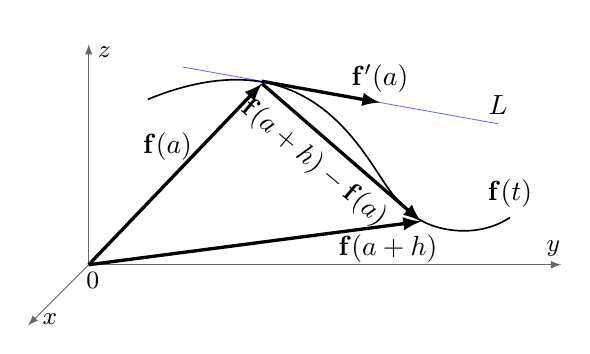
\begin{tikzpicture}
  \usetikzlibrary{arrows}
  \draw [black!60,line width=0.3pt,-latex] (0,0) -- (6,0,0);
  \draw [black!60,line width=0.3pt,-latex] (0,0) -- (0,2.8,0);
  \draw [black!60,line width=0.3pt,-latex] (0,0) -- (0,0,2);
  \pgfputat{\pgfpointxyz{5.9}{0.2}{0}}{\pgfbox[center,center]{\small $y$}};
  \pgfputat{\pgfpointxyz{0.2}{2.7}{0}}{\pgfbox[center,center]{\small $z$}};
  \pgfputat{\pgfpointxyz{0.2}{0}{1.8}}{\pgfbox[center,center]{\small $x$}};
  \pgfputat{\pgfpointxyz{0.05}{-0.2}{0}}{\pgfbox[center,center]{\small $0$}};
  \draw [blue!60,line width=0.3pt] (1.2,2.51) -- (5.2,1.79);
  \draw [rounded corners,line width=0.6pt](0.75,2.1) .. controls (2.95,3) and (3.55,1.2) .. (4,0.75) ..
   controls (4.3,0.45) and (4.9,0.3) .. (5.35,0.6);
  \draw [black,line width=1.2pt,-latex] (0,0) -- (2.2,2.3);
  \draw [black,line width=1.2pt,-latex] (0,0) -- (4.22,0.55);
  \draw [black,line width=1.2pt,-latex] (2.2,2.3) -- (4.22,0.55);
  \draw [black,line width=1.2pt,-latex] (2.2,2.33) -- (3.7,2.06);
  \node [above] at (5.2,1.79) {$L$};
  \node [above] at (5.35,0.6) {$\mathbf{f}(t)$};
  \node [above] at (3.7,2.06) {$\mathbf{f}'(a)$};
  \node [left,above] at (1,1.2) {$\mathbf{f}(a)$};
  \node [below] at (3.8,0.5) {$\mathbf{f}(a + h)$};
  \node [below,rotate=-40] at (3.05,1.52) {$\mathbf{f}(a + h) - \mathbf{f}(a)$};
  \end{tikzpicture}
 \end{center}
 \caption[]{\quad Tangent vector $\mathbf{f}'(a)$ and tangent line $L = \mathbf{f}(a) + s \mathbf{f}'(a)$.}
 \label{fig:vectangent}
\end{figure}
\hrule width \textwidth height 0.5pt
\begin{exmp}
 Let $\mathbf{f}(t) = ( \cos t , \sin t , t )$. Then $\mathbf{f}'(t) = ( -\sin t , \cos t , 1 )$ for all $t$. The
 tangent line $L$ to the curve at $\mathbf{f}(2\pi) = (1,0,2\pi)$ is $L = \mathbf{f}(2\pi) + s\,\mathbf{f}'(2\pi) =
 (1,0,2\pi) + s(0,1,1)$, or in parametric form: $x = 1$, $y = s$, $z = 2\pi + s$ for $-\infty < s < \infty$.
\end{exmp}
\hrule width \textwidth height 0.5pt
\vskip3mm
A \textbf{scalar function}\index{scalar function}\index{function!scalar} is a real-valued function. Note that if
$u(t)$ is a scalar function and $\mathbf{f}(t)$ is a vector-valued function, then their product, defined by
$(u\,\mathbf{f})(t) = u(t)\,\mathbf{f}(t)$ for all $t$, is a vector-valued function (since the product of a scalar
with a vector is a vector).

The basic properties of derivatives of vector-valued functions are summarized in the following theorem.

\statethm{thm:vecdiffprops}{
 {Let $\mathbf{f}(t)$ and $\mathbf{g}(t)$ be differentiable vector-valued functions, let $u(t)$ be a differentiable
 scalar function, let $k$ be a scalar, and let $\mathbf{c}$ be a constant vector. Then\\
 \par\noindent (a) $\dfrac{d}{dt} ( \mathbf{c} ) = \mathbf{0}$;\smallskip
 \par\noindent (b) $\dfrac{d}{dt} ( k \mathbf{f} ) = k \dfrac{d \mathbf{f}}{dt}$;\smallskip
 \par\noindent (c) $\dfrac{d}{dt} ( \mathbf{f} + \mathbf{g} ) = \dfrac{d \mathbf{f}}{dt} \,+\,
  \dfrac{d \mathbf{g}}{dt}$;\smallskip
 \par\noindent (d) $\dfrac{d}{dt} ( \mathbf{f} - \mathbf{g} ) = \dfrac{d \mathbf{f}}{dt} \,-\,
  \dfrac{d \mathbf{g}}{dt}$;\smallskip
 \par\noindent (e) $\dfrac{d}{dt} ( u\,\mathbf{f} ) = \dfrac{du}{dt}\,\mathbf{f} \,+\,
  u \dfrac{d \mathbf{f}}{dt}$;\smallskip
 \par\noindent (f) $\dfrac{d}{dt} ( \Dotprod{\mathbf{f}}{\mathbf{g}} ) = \Dotprod{\dfrac{d \mathbf{f}}{dt}}{\mathbf{g}}
  \,+\, \Dotprod{\mathbf{f}}{\dfrac{d \mathbf{g}}{dt}}$;\smallskip
 \par\noindent (g) $\dfrac{d}{dt} ( \Crossprod{\mathbf{f}\,}{\,\mathbf{g}} ) =
  \Crossprod{\dfrac{d \mathbf{f}}{dt}}{\,\mathbf{g}} \,+\, \Crossprod{\mathbf{f}\,}{\dfrac{d \mathbf{g}}{dt}}$.
 }
}
\begin{proofbar}\begin{proof}[Proof:]
 The proofs of parts (a)--(e) follow easily by differentiating the component functions and using the rules for derivatives from single-variable calculus. 
 We will prove part (f), and leave the proof of part (g) as an exercise for
 the reader.
 \smallskip\\(f)
 Write $\mathbf{f}(t) = ( \ssub{f}{1}(t),\ssub{f}{2}(t),\ssub{f}{3}(t) )$ and
 $\mathbf{g}(t) = ( \ssub{g}{1}(t),\ssub{g}{2}(t),\ssub{g}{3}(t) )$, where the component functions
 $\ssub{f}{1}(t)$, $\ssub{f}{2}(t)$, $\ssub{f}{3}(t)$, $\ssub{g}{1}(t)$, $\ssub{g}{2}(t)$, $\ssub{g}{3}(t)$ are all
 differentiable real-valued functions. Then
 \begin{align*}\begin{split}
  \dfrac{d}{dt} ( \Dotprod{\mathbf{f}(t)}{\mathbf{g}(t)} ) &= \dfrac{d}{dt} ( \ssub{f}{1}(t)\,\ssub{g}{1}(t) +
   \ssub{f}{2}(t)\,\ssub{g}{2}(t) + \ssub{f}{3}(t)\,\ssub{g}{3}(t) )\\
  &= \dfrac{d}{dt} ( \ssub{f}{1}(t)\,\ssub{g}{1}(t) ) +
   \dfrac{d}{dt} ( \ssub{f}{2}(t)\,\ssub{g}{2}(t) ) + \dfrac{d}{dt} ( \ssub{f}{3}(t)\,\ssub{g}{3}(t) )\\
  &= \dfrac{d\ssub{f}{1}}{dt}(t)\,\ssub{g}{1}(t) + \ssub{f}{1}(t)\,\dfrac{d\ssub{g}{1}}{dt}(t) +
   \dfrac{d\ssub{f}{2}}{dt}(t)\,\ssub{g}{2}(t) + \ssub{f}{2}(t)\,\dfrac{d\ssub{g}{2}}{dt}(t) +
   \dfrac{d\ssub{f}{3}}{dt}(t)\,\ssub{g}{3}(t) + \ssub{f}{3}(t)\,\dfrac{d\ssub{g}{3}}{dt}(t)\\
  &= \Dotprod{\biggl( \dfrac{d\ssub{f}{1}}{dt}(t),\dfrac{d\ssub{f}{2}}{dt}(t),\dfrac{d\ssub{f}{3}}{dt}(t) \biggr)}{
   ( \ssub{g}{1}(t),\ssub{g}{2}(t),\ssub{g}{3}(t) )}\\
   &\mathrel{\phantom{=}} {} + \Dotprod{( \ssub{f}{1}(t),\ssub{f}{2}(t),\ssub{f}{3}(t) )}{
   \biggl( \dfrac{d\ssub{g}{1}}{dt}(t),\dfrac{d\ssub{g}{2}}{dt}(t),\dfrac{d\ssub{g}{3}}{dt}(t) \biggr)}\end{split}\\
  &= \Dotprod{\dfrac{d\mathbf{f}}{dt}(t)}{\mathbf{g}(t)} \,+\, \Dotprod{\mathbf{f}(t)}{\dfrac{d\mathbf{g}}{dt}(t)}
   \text{~~for all $t$.} \qedhere
 \end{align*}
\end{proof}\end{proofbar}

\begin{exmp}\label{exmp:absvecderiv}
 Suppose $\mathbf{f}(t)$ is differentiable. Find the derivative of $\norm{\mathbf{f}(t)}$.
 \smallskip
 \par\noindent \emph{Solution:} Since $\norm{\mathbf{f}(t)}$ is a real-valued function of $t$, then by the Chain
 Rule for real-valued functions, we know that
  $\dfrac{d}{dt} \norm{\mathbf{f}(t)}^2 = 2 \norm{\mathbf{f}(t)} \, \dfrac{d}{dt} \norm{\mathbf{f}(t)}$.

 \par\noindent But $\norm{\mathbf{f}(t)}^2 = \Dotprod{\mathbf{f}(t)}{\mathbf{f}(t)}$, so
 $\dfrac{d}{dt} \norm{\mathbf{f}(t)}^2 = \dfrac{d}{dt} ( \Dotprod{\mathbf{f}(t)}{\mathbf{f}(t)} )$.
 Hence, we have
 \begin{align*}
  2 \norm{\mathbf{f}(t)}\,\dfrac{d}{dt} \norm{\mathbf{f}(t)} &= \dfrac{d}{dt} (\Dotprod{\mathbf{f}(t)}{\mathbf{f}(t)})
  = \Dotprod{\mathbf{f}'(t)}{\mathbf{f}(t)} \, + \, \Dotprod{\mathbf{f}(t)}{\mathbf{f}'(t)}
   \text{~~by Theorem \ref{thm:vecdiffprops}(f), so}\\
  &= 2 \Dotprod{\mathbf{f}'(t)}{\mathbf{f}(t)} \text{~,~so if $\norm{\mathbf{f}(t)} \ne 0$ then}\\
  \dfrac{d}{dt} \norm{\mathbf{f}(t)} &= \dfrac{\Dotprod{\mathbf{f}'(t)}{\mathbf{f}(t)}}{\norm{\mathbf{f}(t)}} .
 \end{align*}

We know that $\norm{\mathbf{f}(t)}$ is constant if and only if $\dfrac{d}{dt} \norm{\mathbf{f}(t)} = 0$ for all $t$.
Also, $\mathbf{f}(t) \perp \mathbf{f}'(t)$ if and only if $\Dotprod{\mathbf{f}'(t)}{\mathbf{f}(t)} = 0$. Thus, the
above example shows this important fact:
\begin{center}\statecomment[0.9\textwidth]{
 {\begin{center}If $\norm{\mathbf{f}(t)} \ne 0$, then $\norm{\mathbf{f}(t)}$ is constant if and only if $\mathbf{f}(t)
 \perp \mathbf{f}'(t)$ for all $t$.\end{center}}
}\end{center}
This means that if a curve lies completely on a sphere (or circle) centered at the origin, then the tangent vector
$\mathbf{f}'(t)$ is always perpendicular to the \emph{position vector} $\mathbf{f}(t)$.\index{position vector}
\end{exmp}
\hrule width \textwidth height 0.5pt
\begin{exmp}\label{exmp:sphspiral}
 The \emph{spherical spiral}\index{spherical spiral}
 $\mathbf{f}(t) = \biggl( \dfrac{\cos t}{\sqrt{1 + a^2 t^2}},\dfrac{\sin t}{\sqrt{1 + a^2 t^2}},
  \dfrac{-at}{\sqrt{1 + a^2 t^2}} \biggr)$, for $a \ne 0$.\smallskip
  \par\noindent Figure \ref{fig:sphspiral} shows the graph of the curve when $a = 0.2$. In the exercises, the reader will be asked to
  show that this curve lies on the sphere $x^2 + y^2 + z^2 = 1$ and to verify directly that
  $\Dotprod{\mathbf{f}'(t)}{\mathbf{f}(t)} = 0$ for all $t$.
 \begin{figure}[h]
  \begin{center}
   % GNUPLOT: LaTeX picture with Postscript
\begingroup
\scriptsize
  \makeatletter
  \providecommand\color[2][]{%
    \GenericError{(gnuplot) \space\space\space\@spaces}{%
      Package color not loaded in conjunction with
      terminal option `colourtext'%
    }{See the gnuplot documentation for explanation.%
    }{Either use 'blacktext' in gnuplot or load the package
      color.sty in LaTeX.}%
    \renewcommand\color[2][]{}%
  }%
  \providecommand\includegraphics[2][]{%
    \GenericError{(gnuplot) \space\space\space\@spaces}{%
      Package graphicx or graphics not loaded%
    }{See the gnuplot documentation for explanation.%
    }{The gnuplot epslatex terminal needs graphicx.sty or graphics.sty.}%
    \renewcommand\includegraphics[2][]{}%
  }%
  \providecommand\rotatebox[2]{#2}%
  \@ifundefined{ifGPcolor}{%
    \newif\ifGPcolor
    \GPcolortrue
  }{}%
  \@ifundefined{ifGPblacktext}{%
    \newif\ifGPblacktext
    \GPblacktexttrue
  }{}%
  % define a \g@addto@macro without @ in the name:
  \let\gplgaddtomacro\g@addto@macro
  % define empty templates for all commands taking text:
  \gdef\gplbacktext{}%
  \gdef\gplfronttext{}%
  \makeatother
  \ifGPblacktext
    % no textcolor at all
    \def\colorrgb#1{}%
    \def\colorgray#1{}%
  \else
    % gray or color?
    \ifGPcolor
      \def\colorrgb#1{\color[rgb]{#1}}%
      \def\colorgray#1{\color[gray]{#1}}%
      \expandafter\def\csname LTw\endcsname{\color{white}}%
      \expandafter\def\csname LTb\endcsname{\color{black}}%
      \expandafter\def\csname LTa\endcsname{\color{black}}%
      \expandafter\def\csname LT0\endcsname{\color[rgb]{1,0,0}}%
      \expandafter\def\csname LT1\endcsname{\color[rgb]{0,1,0}}%
      \expandafter\def\csname LT2\endcsname{\color[rgb]{0,0,1}}%
      \expandafter\def\csname LT3\endcsname{\color[rgb]{1,0,1}}%
      \expandafter\def\csname LT4\endcsname{\color[rgb]{0,1,1}}%
      \expandafter\def\csname LT5\endcsname{\color[rgb]{1,1,0}}%
      \expandafter\def\csname LT6\endcsname{\color[rgb]{0,0,0}}%
      \expandafter\def\csname LT7\endcsname{\color[rgb]{1,0.3,0}}%
      \expandafter\def\csname LT8\endcsname{\color[rgb]{0.5,0.5,0.5}}%
    \else
      % gray
      \def\colorrgb#1{\color{black}}%
      \def\colorgray#1{\color[gray]{#1}}%
      \expandafter\def\csname LTw\endcsname{\color{white}}%
      \expandafter\def\csname LTb\endcsname{\color{black}}%
      \expandafter\def\csname LTa\endcsname{\color{black}}%
      \expandafter\def\csname LT0\endcsname{\color{black}}%
      \expandafter\def\csname LT1\endcsname{\color{black}}%
      \expandafter\def\csname LT2\endcsname{\color{black}}%
      \expandafter\def\csname LT3\endcsname{\color{black}}%
      \expandafter\def\csname LT4\endcsname{\color{black}}%
      \expandafter\def\csname LT5\endcsname{\color{black}}%
      \expandafter\def\csname LT6\endcsname{\color{black}}%
      \expandafter\def\csname LT7\endcsname{\color{black}}%
      \expandafter\def\csname LT8\endcsname{\color{black}}%
    \fi
  \fi
  \setlength{\unitlength}{0.0500bp}%
  \begin{picture}(6802.00,5040.00)%
    \gplgaddtomacro\gplbacktext{%
      \csname LTb\endcsname%
      \put(5969,1764){\makebox(0,0)[l]{\strut{}-1}}%
      \put(5793,1661){\makebox(0,0)[l]{\strut{}-0.8}}%
      \put(5618,1558){\makebox(0,0)[l]{\strut{}-0.6}}%
      \put(5442,1455){\makebox(0,0)[l]{\strut{}-0.4}}%
      \put(5266,1353){\makebox(0,0)[l]{\strut{}-0.2}}%
      \put(5091,1250){\makebox(0,0)[l]{\strut{} 0}}%
      \put(4915,1147){\makebox(0,0)[l]{\strut{} 0.2}}%
      \put(4739,1044){\makebox(0,0)[l]{\strut{} 0.4}}%
      \put(4564,941){\makebox(0,0)[l]{\strut{} 0.6}}%
      \put(4388,838){\makebox(0,0)[l]{\strut{} 0.8}}%
      \put(4212,735){\makebox(0,0)[l]{\strut{} 1}}%
      \put(936,1320){\makebox(0,0){\strut{}-1}}%
      \put(1240,1260){\makebox(0,0){\strut{}-0.8}}%
      \put(1545,1201){\makebox(0,0){\strut{}-0.6}}%
      \put(1849,1142){\makebox(0,0){\strut{}-0.4}}%
      \put(2153,1082){\makebox(0,0){\strut{}-0.2}}%
      \put(2457,1023){\makebox(0,0){\strut{} 0}}%
      \put(2761,963){\makebox(0,0){\strut{} 0.2}}%
      \put(3066,904){\makebox(0,0){\strut{} 0.4}}%
      \put(3370,845){\makebox(0,0){\strut{} 0.6}}%
      \put(3673,785){\makebox(0,0){\strut{} 0.8}}%
      \put(3977,726){\makebox(0,0){\strut{} 1}}%
      \put(876,1384){\makebox(0,0)[r]{\strut{}-1}}%
      \put(876,1590){\makebox(0,0)[r]{\strut{}-0.8}}%
      \put(876,1796){\makebox(0,0)[r]{\strut{}-0.6}}%
      \put(876,2002){\makebox(0,0)[r]{\strut{}-0.4}}%
      \put(876,2207){\makebox(0,0)[r]{\strut{}-0.2}}%
      \put(876,2413){\makebox(0,0)[r]{\strut{} 0}}%
      \put(876,2619){\makebox(0,0)[r]{\strut{} 0.2}}%
      \put(876,2824){\makebox(0,0)[r]{\strut{} 0.4}}%
      \put(876,3029){\makebox(0,0)[r]{\strut{} 0.6}}%
      \put(876,3235){\makebox(0,0)[r]{\strut{} 0.8}}%
      \put(876,3441){\makebox(0,0)[r]{\strut{} 1}}%
      \put(-185,2633){\makebox(0,0){\strut{}$z$}}%
    }%
    \gplgaddtomacro\gplfronttext{%
      \csname LTb\endcsname%
      \put(5682,1156){\makebox(0,0){\strut{}$x$}}%
      \put(2084,830){\makebox(0,0){\strut{}$y$}}%
      \put(-185,2633){\makebox(0,0){\strut{}$z$}}%
    }%
    \gplbacktext
    \put(0,0){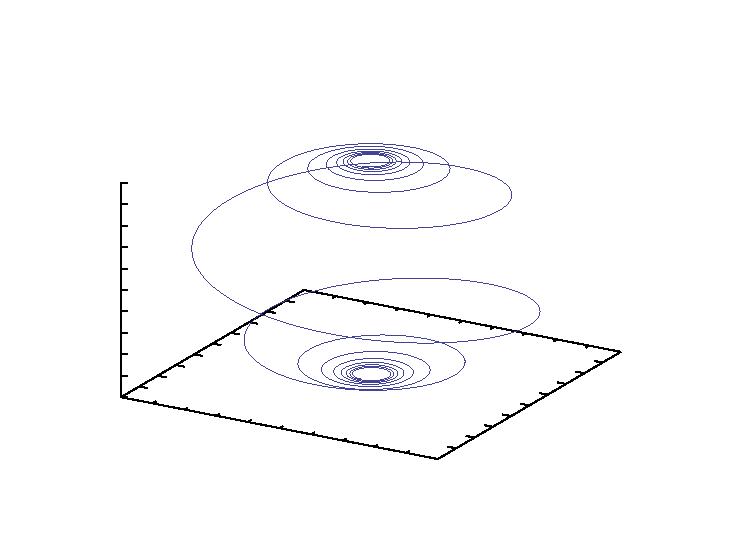
\includegraphics{fig183}}%
    \gplfronttext
  \end{picture}%
\endgroup

  \end{center}
 \caption[]{\quad Spherical spiral with $a = 0.2$.}
 \label{fig:sphspiral}
 \end{figure}
\end{exmp}
\hrule width \textwidth height 0.5pt
\vskip3mm
Just as in single-variable calculus, higher-order derivatives of vector-valued functions are obtained by repeatedly
differentiating the (first) derivative of the function:
\begin{displaymath}
 \mathbf{f}''(t) = \dfrac{d}{dt} \mathbf{f}'(t) \; , \qquad \mathbf{f}'''(t) = \dfrac{d}{dt} \mathbf{f}''(t) \;
 , \quad \ldots \quad , \quad \dfrac{d^{n}\mathbf{f}}{dt^{n}} =
 \dfrac{d}{dt} \biggl( \dfrac{d^{n-1}\mathbf{f}}{dt^{n-1}} \biggr) \text{~~~(for $n = 2, 3, 4,\ldots$).}
\end{displaymath}

We can use vector-valued functions to represent physical quantities, such as velocity, acceleration, force, momentum, etc. 
For example, let the real variable $t$ represent time elapsed from some initial time ($t = 0$), and suppose
that an object of constant mass $m$ is subjected to some force so that it moves in space, with its position $(x,y,z)$ at
time $t$ a function of $t$. That is, $x = x(t)$, $y = y(t)$, $z = z(t)$ for some real-valued functions $x(t)$, $y(t)$,
$z(t)$. Call $\mathbf{r}(t) = (x(t),y(t),z(t))$ the \textbf{position vector}\index{position vector} of the object. We
can define various physical quantities associated with the object as follows:\footnote{We will often use the
older dot notation for derivatives when physics is involved.}
\begin{align*}
 \text{\emph{position}: } \mathbf{r}(t) &= (x(t),y(t),z(t));\\
 \text{\emph{velocity}: } \mathbf{v}(t) &= \dot{\mathbf{r}}(t) = \mathbf{r}'(t) = \dfrac{d \mathbf{r}}{dt}\\
 &= (x'(t),y'(t),z'(t));\\
 \text{\emph{acceleration}: } \mathbf{a}(t) &= \dot{\mathbf{v}}(t) = \mathbf{v}'(t) = \dfrac{d \mathbf{v}}{dt}\\
 &= \ddot{\mathbf{r}}(t) = \mathbf{r}''(t) = \dfrac{d^2 \mathbf{r}}{dt^2}\\
 &= (x''(t),y''(t),z''(t));\\
 \text{\emph{momentum}: } \mathbf{p}(t) &= m \mathbf{v}(t);\\
 \text{\emph{force}: } \mathbf{F}(t) &= \dot{\mathbf{p}}(t) = \mathbf{p}'(t) = \dfrac{d \mathbf{p}}{dt}
 \text{~~~~(Newton's Second Law of Motion).}
\end{align*}
The magnitude $\norm{\mathbf{v}(t)}$ of the velocity vector is called the \emph{speed} of the object.
Note that since the mass $m$ is a constant, the force equation becomes the familiar
$\mathbf{F}(t) = m \mathbf{a}(t)$.\index{velocity}\index{acceleration}\index{momentum}\index{force}

\smallskip
\hrule width \textwidth height 0.5pt
\begin{exmp}
 Let $\mathbf{r}(t) = (5 \cos t , 3 \sin t , 4 \sin t )$ be the position vector of an object at time $t \ge 0$. Find
 its (a) velocity and (b) acceleration vectors.
 \smallskip
 \par\noindent \emph{Solution:} (a) $\mathbf{v}(t) = \dot{\mathbf{r}}(t) = (-5 \sin t , 3 \cos t ,
 4 \cos t )$.
 \smallskip
 \par\noindent (b) $\mathbf{a}(t) = \dot{\mathbf{v}}(t) = (-5 \cos t , -3 \sin t , -4 \sin t )$.
 \smallskip
 
 \par\noindent Note that $\norm{\mathbf{r}(t)} = \sqrt{25 \cos^2 t + 25 \sin^2 t} = 5$ for all $t$, so by Example
 \ref{exmp:absvecderiv} we know that $\Dotprod{\mathbf{r}(t)}{\dot{\mathbf{r}}(t)} = 0$ for all $t$ (which we can verify
 from part (a)). In fact, $\norm{\mathbf{v}(t)} = 5$ for all $t$ also. And not only does $\mathbf{r}(t)$ lie on the
 sphere of radius $5$ centered at the origin, but perhaps not so obvious is that it lies completely within a
 \emph{circle} of radius 5 centered at the origin. Also, note that $\mathbf{a}(t) = -\mathbf{r}(t)$. It turns out (see
 Exercise 16) that whenever an object moves in a circle with constant speed, the acceleration vector will point towards the center of the circle.
\end{exmp}
\hrule width \textwidth height 0.5pt
\vskip3mm

Recall from Section 1.5 that if $\ssub{\mathbf{r}}{1}$, $\ssub{\mathbf{r}}{2}$ are position vectors to distinct points
then $\ssub{\mathbf{r}}{1} + t (\ssub{\mathbf{r}}{2} - \ssub{\mathbf{r}}{1})$ represents a line through those two
points as $t$ varies over all real numbers. That vector sum can be written as $(1 - t) \ssub{\mathbf{r}}{1} +
t \ssub{\mathbf{r}}{2}$. So the function $\mathbf{l}(t) = (1 - t) \ssub{\mathbf{r}}{1} +
t \ssub{\mathbf{r}}{2}$ is a line through the terminal points of $\ssub{\mathbf{r}}{1}$ and $\ssub{\mathbf{r}}{2}$, and
when $t$ is restricted to the interval $\left[ 0,1 \right]$ it is the line segment between the points, with
$\mathbf{l}(0) = \ssub{\mathbf{r}}{1}$ and $\mathbf{l}(1) = \ssub{\mathbf{r}}{2}$.

In general, a function of the form
$\mathbf{f}(t) = (\ssub{a}{1}t + \ssub{b}{1},\ssub{a}{2}t + \ssub{b}{2},\ssub{a}{3}t + \ssub{b}{3})$ represents a line
in $\Real{3}$. A function of the form
$\mathbf{f}(t) = (\ssub{a}{1}t^2 + \ssub{b}{1}t + \ssub{c}{1},\ssub{a}{2}t^2 + \ssub{b}{2}t + \ssub{c}{2},
\ssub{a}{3}t^2 + \ssub{b}{3}t + \ssub{c}{3})$ represents a (possibly degenerate) parabola in $\Real{3}$.

\smallskip
\hrule width \textwidth height 0.5pt
\begin{exmp}\label{exmp:bezier}
 \emph{B\'{e}zier curves}\index{B\'{e}zier curve} are used in Computer Aided Design to approximate the shape of a
 polygonal path in space (called the \emph{B\'{e}zier polygon} or \emph{control polygon}). For instance, given three
 points (or position vectors) $\ssub{\mathbf{b}}{0}$, $\ssub{\mathbf{b}}{1}$, $\ssub{\mathbf{b}}{2}$ in $\Real{3}$,
 define
 \begin{align*}
  \ssub{\mathbf{b}}{0}^{\scriptscriptstyle 1}(t) &= ( 1 - t )\ssub{\mathbf{b}}{0} + t \ssub{\mathbf{b}}{1},\\
  \ssub{\mathbf{b}}{1}^{\scriptscriptstyle 1}(t) &= ( 1 - t )\ssub{\mathbf{b}}{1} + t \ssub{\mathbf{b}}{2},
  \\
  \ssub{\mathbf{b}}{0}^{\scriptscriptstyle 2}(t) &=
  ( 1 - t )\ssub{\mathbf{b}}{0}^{\scriptscriptstyle 1}(t) + t \ssub{\mathbf{b}}{1}^{\scriptscriptstyle 1}(t)\\
  &= (1 - t)^2 \ssub{\mathbf{b}}{0} + 2t(1 - t) \ssub{\mathbf{b}}{1} + t^2 \ssub{\mathbf{b}}{2}
 \end{align*}
 for all real $t$. For $t$ in the interval $[0,1]$, we see that $\ssub{\mathbf{b}}{0}^{\scriptscriptstyle 1}(t)$ is the
 line segment between $\ssub{\mathbf{b}}{0}$ and $\ssub{\mathbf{b}}{1}$, and
 $\ssub{\mathbf{b}}{1}^{\scriptscriptstyle 1}(t)$ is the line segment between $\ssub{\mathbf{b}}{1}$ and
 $\ssub{\mathbf{b}}{2}$. The function $\ssub{\mathbf{b}}{0}^{\scriptscriptstyle 2}(t)$ is the
 B\'{e}zier curve for the points $\ssub{\mathbf{b}}{0}$, $\ssub{\mathbf{b}}{1}$, $\ssub{\mathbf{b}}{2}$. Note from the
 last formula that the curve is a parabola that goes through $\ssub{\mathbf{b}}{0}$ (when $t = 0$) and
 $\ssub{\mathbf{b}}{2}$ (when $t = 1$).
 
 As an example, let $\ssub{\mathbf{b}}{0} = (0,0,0)$, $\ssub{\mathbf{b}}{1} = (1,2,3)$, and $\ssub{\mathbf{b}}{2} =
 (4,5,2)$. Then the explicit formula for the B\'{e}zier curve is
 $\ssub{\mathbf{b}}{0}^{\scriptscriptstyle 2}(t) = ( 2t + 2t^2, 4t + t^2, 6t - 4t^2 )$, as shown in Figure
 \ref{fig:bezier2}, where the line segments are $\ssub{\mathbf{b}}{0}^{\scriptscriptstyle 1}(t)$ and
 $\ssub{\mathbf{b}}{1}^{\scriptscriptstyle 1}(t)$, and the curve is
 $\ssub{\mathbf{b}}{0}^{\scriptscriptstyle 2}(t)$.
 \begin{figure}[h]
  \begin{center}
   \input{fig184}
  \end{center}
 \caption[]{\quad B\'{e}zier curve approximation for three points.}
 \label{fig:bezier2}
 \end{figure}

 In general, the polygonal path determined by $n \ge 3$ noncollinear points in $\Real{3}$ can be used to define
 the B\'{e}zier curve recursively by a process called \emph{repeated linear interpolation}. This curve will be a
 vector-valued function whose components are polynomials of degree $n-1$, and its formula is given by
 \emph{de Casteljau's algorithm}.\footnote{See pp. 27--30 in \cite{far}.} In the exercises, the reader will be given the
 algorithm for the case of $n = 4$ points and asked to write the explicit formula for the B\'{e}zier curve for the four
 points shown in Figure \ref{fig:bezier3}.
\end{exmp}

\hrule width \textwidth height 0.5pt
\smallskip

\begin{exmp}
The \emph{pedal curve} is traced by the orthogonal projection of a fixed point $P$ on the tangent lines of a given curve $\mathbf{f}(t)$.
\end{exmp}

Write a parametric expression $\mathbf{h}(t)$ for the pedal curve for the unit circle $\mathbf{f}(t)=(\cos(t),\sin t)$ and the point $P=(1,0)$, so its position vector is $\mathbf{i}$. (This curve is called cardioid.)

\begin{wrapfigure}{r}{32 mm}
\begin{lpic}[t(-0 mm),b(0 mm),r(0 mm),l(0 mm)]{pics/pedal-curve(1)}
\lbl[rt]{22.5,15.5;$P$}
\end{lpic}
\end{wrapfigure}

Denote by $\mathbf{w}(t)$ the projection of $\mathbf{v}(t)=\mathbf{i}-\mathbf{f}(t)$ to the tangent line at $\mathbf{f}(t)$, so $\mathbf{h}(t)=\mathbf{f}(t)+\mathbf{w}(t)$.

The velocity vector $\mathbf{f}'(t)=(-\sin t,\cos t)$ is parallel to the tangent line at $\mathbf{f}(t)$.

Note that $\|\mathbf{f}'(t)\|=1$ for any $t$.
Therefore the vector $\mathbf{w}(t)$ can be found useing the following formula (compare to  Example~\ref{exmp:projection} and Exercise~\ref{ex:projection}, on page~\pageref{ex:projection})
\begin{align*}
\mathbf{w}(t)
&=
(\mathbf{f}'(t)\cdot\mathbf{v}(t))\,\mathbf{f}'(t)
\\
&=(\mathbf{f}'(t)\cdot(\mathbf{i}-\mathbf{f}(t)))\,\mathbf{f}'(t)
\\
&=(\sin^2 t,-\sin t\cos t).
\intertext{and} 
\mathbf{h}(t)
&=\mathbf{f}(t)+\mathbf{w}(t)
\\
&=(\cos t+\sin^2t,\sin t-\sin t\cos t).
\end{align*}


\startexercises\label{sec1dot8}
\probs{A}
\par\noindent For Exercises 1--4, calculate $\mathbf{f}'(t)$ and find the tangent line at $\mathbf{f}(0)$.
\begin{enumerate}[\bfseries 1.]
 \begin{multicols}{2}
  \item $\mathbf{f}(t) = (t + 1 , t^2 + 1 , t^3 + 1)$;
  \item $\mathbf{f}(t) = (e^t + 1 , e^{2t} + 1 , e^{t^2} + 1)$;
 \end{multicols}
 \begin{multicols}{2}
  \item $\mathbf{f}(t) = (\cos 2t , \sin 2t , t)$;
  \item $\mathbf{f}(t) = (\sin 2t , 2\sin^2 t , 2\cos t)$.
 \end{multicols}
\suspend{enumerate}
\par\noindent For Exercises 5--6, find the velocity $\mathbf{v}(t)$ and acceleration $\mathbf{a}(t)$ of an object
with the given position vector $\mathbf{r}(t)$.
\resume{enumerate}[{[\bfseries 1.]}]
 \begin{multicols}{2}
  \item $\mathbf{r}(t) = (t, t - \sin t , 1 - \cos t)$;
  \item $\mathbf{r}(t) = (3\cos t , 2\sin t , 1)$.
 \end{multicols}
\suspend{enumerate}
\probs{B}
\resume{enumerate}[{[\bfseries 1.]}]
 \item Let $\mathbf{f}(t) = \biggl( \dfrac{\cos t}{\sqrt{1 + a^2 t^2}},\dfrac{\sin t}{\sqrt{1 + a^2 t^2}},
  \dfrac{-at}{\sqrt{1 + a^2 t^2}} \biggr)$, with $a \ne 0$.
  \begin{enumerate}[(a)]
   \item Show that $\norm{\mathbf{f}(t)} = 1$ for all $t$.
   \item Show directly that $\Dotprod{\mathbf{f}'(t)}{\mathbf{f}(t)} = 0$ for all $t$.
  \end{enumerate}
 \item If $\mathbf{f}'(t) = \mathbf{0}$ for all $t$ in some interval $(a,b)$, show that $\mathbf{f}(t)$ is
  a constant vector in $(a,b)$.
 \item For a constant vector $\mathbf{c} \ne \mathbf{0}$, the function $\mathbf{f}(t) = t\mathbf{c}$ represents a line
  parallel to $\mathbf{c}$.
  \begin{enumerate}[(a)]
   \item What kind of curve does $\mathbf{g}(t) = t^3\mathbf{c}$ represent? Explain.
   \item What kind of curve does $\mathbf{h}(t) = e^t\mathbf{c}$ represent? Explain.
   \item Compare $\mathbf{f}'(0)$ and $\mathbf{g}'(0)$. 
   Given your answer to part (a), how do you explain the difference in the two derivatives?
  \end{enumerate}
 \item Show that 
 \[\dfrac{d}{dt} \biggl( \Crossprod{\mathbf{f}\,}{\dfrac{d\mathbf{f}}{dt}} \biggr) =
  \Crossprod{\mathbf{f}\,}{\dfrac{d^2 \mathbf{f}}{dt^2}}.\]
 \item Let a particle of (constant) mass $m$ have position vector $\mathbf{r}(t)$, velocity $\mathbf{v}(t)$,
  acceleration $\mathbf{a}(t)$ and momentum $\mathbf{p}(t)$ at time $t$. The \emph{angular momentum} $\mathbf{L}(t)$ of
  the particle with respect to the origin at time $t$ is defined as $\mathbf{L}(t) =
  \Crossprod{\mathbf{r}(t)}{\,\mathbf{p}(t)}$. 
  If $\mathbf{F}(t)$ is the force acting on the particle at time $t$, then
  define the \emph{torque} $\mathbf{N}(t)$ acting on the particle with respect to the origin as
  $\mathbf{N}(t) = \Crossprod{\mathbf{r}(t)}{\mathbf{F}(t)}$. Show that $\mathbf{L}'(t) = \mathbf{N}(t)$.
 \item Show that $\dfrac{d}{dt} ( \Dotprod{\mathbf{f}}{( \Crossprod{\mathbf{g}\,}{\,\mathbf{h}} )} ) =
  \Dotprod{\dfrac{d\mathbf{f}}{dt}}{(\Crossprod{\mathbf{g}\,}{\,\mathbf{h}})} \,+\,
  \Dotprod{\mathbf{f}}{\biggl(\Crossprod{\dfrac{d \mathbf{g}}{dt}}{\,\mathbf{h}}\biggr)} \,+\,
  \Dotprod{\mathbf{f}}{\biggl(\Crossprod{\mathbf{g}\,}{\dfrac{d \mathbf{h}}{dt}}\biggr)}$.
 \item The Mean Value Theorem does not hold for vector-valued functions:
 Show that for $\mathbf{f}(t) = (\cos t, \sin t,t)$, there is no $t$ in the interval $(0,2\pi)$ such that
 \begin{displaymath}
  \mathbf{f}'(t) = \dfrac{\mathbf{f}(2\pi) - \mathbf{f}(0)}{2\pi - 0} .
 \end{displaymath}
 \item Wrie a parametric equation for the pedal curve to $\mathbf{f}(t)=(t,t^2,t^3)$ with respect to the origin.
\suspend{enumerate}
\probs{C}
\resume{enumerate}[{[\bfseries 1.]}]
 \item The B\'{e}zier curve $\ssub{\mathbf{b}}{0}^{\scriptscriptstyle 3}(t)$ for four noncollinear points
  $\ssub{\mathbf{b}}{0}$, $\ssub{\mathbf{b}}{1}$, $\ssub{\mathbf{b}}{2}$, $\ssub{\mathbf{b}}{3}$ in $\Real{3}$ is
  defined by the following algorithm (going from the left column to the right):
  \begin{alignat*}{3}
   \ssub{\mathbf{b}}{0}^{\scriptscriptstyle 1}(t) &= ( 1 - t )\ssub{\mathbf{b}}{0} + t \ssub{\mathbf{b}}{1},
    \\
   \ssub{\mathbf{b}}{1}^{\scriptscriptstyle 1}(t) &= ( 1 - t )\ssub{\mathbf{b}}{1} + t \ssub{\mathbf{b}}{2}, \qquad
    & \ssub{\mathbf{b}}{0}^{\scriptscriptstyle 2}(t) &=
    ( 1 - t )\ssub{\mathbf{b}}{0}^{\scriptscriptstyle 1}(t) + t \ssub{\mathbf{b}}{1}^{\scriptscriptstyle 1}(t),
    \\
   \ssub{\mathbf{b}}{2}^{\scriptscriptstyle 1}(t) &= ( 1 - t )\ssub{\mathbf{b}}{2} + t \ssub{\mathbf{b}}{3}.\qquad
    & \ssub{\mathbf{b}}{1}^{\scriptscriptstyle 2}(t) &=
    ( 1 - t )\ssub{\mathbf{b}}{1}^{\scriptscriptstyle 1}(t) + t \ssub{\mathbf{b}}{2}^{\scriptscriptstyle 1}(t),\qquad
    & \ssub{\mathbf{b}}{0}^{\scriptscriptstyle 3}(t) &=
    ( 1 - t )\ssub{\mathbf{b}}{0}^{\scriptscriptstyle 2}(t) + t \ssub{\mathbf{b}}{1}^{\scriptscriptstyle 2}(t).
  \end{alignat*}
  \begin{enumerate}[(a)]
   \item Show that $\ssub{\mathbf{b}}{0}^{\scriptscriptstyle 3}(t) = (1 - t)^3 \ssub{\mathbf{b}}{0} +
    3t(1 - t)^2 \ssub{\mathbf{b}}{1} + 3t^2 (1 - t) \ssub{\mathbf{b}}{2} + t^3 \ssub{\mathbf{b}}{3}$.
   \item Write the explicit formula (as in Example \ref{exmp:bezier}) for the B\'{e}zier curve for the points
   $\ssub{\mathbf{b}}{0} = (0,0,0)$, $\ssub{\mathbf{b}}{1} = (0,1,1)$, $\ssub{\mathbf{b}}{2} = (2,3,0)$,
   $\ssub{\mathbf{b}}{3} = (4,5,2)$.
  \end{enumerate}
\item 
Let $\mathbf{r}(t)$ be the position vector for a particle moving in $\Real{3}$,
$\mathbf{v}(t)$ be its velocity 
and $\mathbf{a}(t)$ be its acceleration.
Show that
  \begin{displaymath}
   \dfrac{d}{dt} ( \Crossprod{\mathbf{r}}{( \Crossprod{\mathbf{v}\,}{\,\mathbf{r}} )} ) =
    \norm{\mathbf{r}}^2 \mathbf{a} + (\Dotprod{\mathbf{r}}{\mathbf{v}}) \mathbf{v} -
    (\norm{\mathbf{v}}^2 + \Dotprod{\mathbf{r}}{\mathbf{a}})\mathbf{r}.
  \end{displaymath} 
\item 
Let $\mathbf{r}(t)$ be the position vector in $\Real{3}$ for a particle that moves with constant speed $c > 0$ in a circle of radius $a > 0$ centered at the origin in the $xy$-plane. 
Show that its acceleration $\mathbf{a}(t)$ points in the opposite direction as
  $\mathbf{r}(t)$ for all $t$. (\emph{Hint: Use Example \ref{exmp:absvecderiv} to show that} $\mathbf{r}(t)
  \perp \mathbf{v}(t)$ \emph{and} $\mathbf{a}(t) \perp \mathbf{v}(t)$, \emph{and hence} $\mathbf{a}(t) \parallel
  \mathbf{r}(t)$.)
 \item Prove Theorem \ref{thm:vecdiffprops}(g).
 
 \item Show that there is no plane which is \emph{tangent}\footnote{A plane is called tangent to a curve $\mathbf{f}(t)$ at point $\mathbf{f}(t_0)$ it it contains the tangent line at $\mathbf{f}(t_0)$.} to the curve $\mathbf{f}(t)=(t,t^2,t^3)$ at two distinct points.
\end{enumerate}
\begin{figure}[h]
  \begin{center}
   % GNUPLOT: LaTeX picture with Postscript
\begingroup
\scriptsize
  \makeatletter
  \providecommand\color[2][]{%
    \GenericError{(gnuplot) \space\space\space\@spaces}{%
      Package color not loaded in conjunction with
      terminal option `colourtext'%
    }{See the gnuplot documentation for explanation.%
    }{Either use 'blacktext' in gnuplot or load the package
      color.sty in LaTeX.}%
    \renewcommand\color[2][]{}%
  }%
  \providecommand\includegraphics[2][]{%
    \GenericError{(gnuplot) \space\space\space\@spaces}{%
      Package graphicx or graphics not loaded%
    }{See the gnuplot documentation for explanation.%
    }{The gnuplot epslatex terminal needs graphicx.sty or graphics.sty.}%
    \renewcommand\includegraphics[2][]{}%
  }%
  \providecommand\rotatebox[2]{#2}%
  \@ifundefined{ifGPcolor}{%
    \newif\ifGPcolor
    \GPcolortrue
  }{}%
  \@ifundefined{ifGPblacktext}{%
    \newif\ifGPblacktext
    \GPblacktexttrue
  }{}%
  % define a \g@addto@macro without @ in the name:
  \let\gplgaddtomacro\g@addto@macro
  % define empty templates for all commands taking text:
  \gdef\gplbacktext{}%
  \gdef\gplfronttext{}%
  \makeatother
  \ifGPblacktext
    % no textcolor at all
    \def\colorrgb#1{}%
    \def\colorgray#1{}%
  \else
    % gray or color?
    \ifGPcolor
      \def\colorrgb#1{\color[rgb]{#1}}%
      \def\colorgray#1{\color[gray]{#1}}%
      \expandafter\def\csname LTw\endcsname{\color{white}}%
      \expandafter\def\csname LTb\endcsname{\color{black}}%
      \expandafter\def\csname LTa\endcsname{\color{black}}%
      \expandafter\def\csname LT0\endcsname{\color[rgb]{1,0,0}}%
      \expandafter\def\csname LT1\endcsname{\color[rgb]{0,1,0}}%
      \expandafter\def\csname LT2\endcsname{\color[rgb]{0,0,1}}%
      \expandafter\def\csname LT3\endcsname{\color[rgb]{1,0,1}}%
      \expandafter\def\csname LT4\endcsname{\color[rgb]{0,1,1}}%
      \expandafter\def\csname LT5\endcsname{\color[rgb]{1,1,0}}%
      \expandafter\def\csname LT6\endcsname{\color[rgb]{0,0,0}}%
      \expandafter\def\csname LT7\endcsname{\color[rgb]{1,0.3,0}}%
      \expandafter\def\csname LT8\endcsname{\color[rgb]{0.5,0.5,0.5}}%
    \else
      % gray
      \def\colorrgb#1{\color{black}}%
      \def\colorgray#1{\color[gray]{#1}}%
      \expandafter\def\csname LTw\endcsname{\color{white}}%
      \expandafter\def\csname LTb\endcsname{\color{black}}%
      \expandafter\def\csname LTa\endcsname{\color{black}}%
      \expandafter\def\csname LT0\endcsname{\color{black}}%
      \expandafter\def\csname LT1\endcsname{\color{black}}%
      \expandafter\def\csname LT2\endcsname{\color{black}}%
      \expandafter\def\csname LT3\endcsname{\color{black}}%
      \expandafter\def\csname LT4\endcsname{\color{black}}%
      \expandafter\def\csname LT5\endcsname{\color{black}}%
      \expandafter\def\csname LT6\endcsname{\color{black}}%
      \expandafter\def\csname LT7\endcsname{\color{black}}%
      \expandafter\def\csname LT8\endcsname{\color{black}}%
    \fi
  \fi
  \setlength{\unitlength}{0.0500bp}%
  \begin{picture}(6802.00,5040.00)%
    \gplgaddtomacro\gplbacktext{%
      \csname LTb\endcsname%
      \put(5835,1731){\makebox(0,0)[l]{\strut{} 0}}%
      \put(5685,1636){\makebox(0,0)[l]{\strut{} 0.5}}%
      \put(5535,1540){\makebox(0,0)[l]{\strut{} 1}}%
      \put(5385,1445){\makebox(0,0)[l]{\strut{} 1.5}}%
      \put(5234,1349){\makebox(0,0)[l]{\strut{} 2}}%
      \put(5084,1254){\makebox(0,0)[l]{\strut{} 2.5}}%
      \put(4934,1159){\makebox(0,0)[l]{\strut{} 3}}%
      \put(4784,1063){\makebox(0,0)[l]{\strut{} 3.5}}%
      \put(4634,968){\makebox(0,0)[l]{\strut{} 4}}%
      \put(1105,1223){\makebox(0,0){\strut{} 0}}%
      \put(1765,1168){\makebox(0,0){\strut{} 1}}%
      \put(2425,1112){\makebox(0,0){\strut{} 2}}%
      \put(3086,1057){\makebox(0,0){\strut{} 3}}%
      \put(3745,1001){\makebox(0,0){\strut{} 4}}%
      \put(4405,946){\makebox(0,0){\strut{} 5}}%
      \put(1024,1271){\makebox(0,0)[r]{\strut{} 0}}%
      \put(1024,1829){\makebox(0,0)[r]{\strut{} 0.5}}%
      \put(1024,2388){\makebox(0,0)[r]{\strut{} 1}}%
      \put(1024,2945){\makebox(0,0)[r]{\strut{} 1.5}}%
      \put(1024,3503){\makebox(0,0)[r]{\strut{} 2}}%
      \put(455,2197){\makebox(0,0){\strut{}$z$}}%
    }%
    \gplgaddtomacro\gplfronttext{%
      \csname LTb\endcsname%
      \put(5876,1306){\makebox(0,0){\strut{}$x$}}%
      \put(2830,832){\makebox(0,0){\strut{}$y$}}%
      \put(455,2197){\makebox(0,0){\strut{}$z$}}%
      \put(1855,2065){\makebox(0,0)[l]{\strut{}$(0,0,0)$}}%
      \put(3042,3126){\makebox(0,0)[l]{\strut{}$(0,1,1)$}}%
      \put(3762,1516){\makebox(0,0)[l]{\strut{}$(2,3,0)$}}%
      \put(4481,3256){\makebox(0,0)[l]{\strut{}$(4,5,2)$}}%
    }%
    \gplbacktext
    \put(0,0){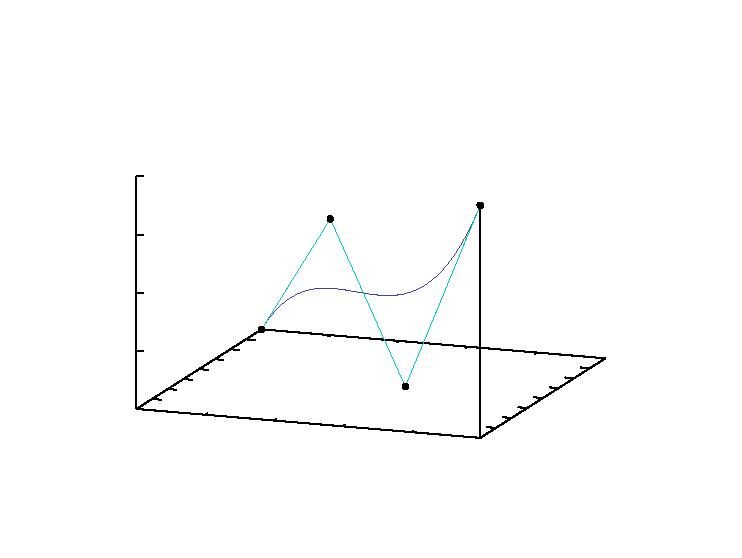
\includegraphics{fig185}}%
    \gplfronttext
  \end{picture}%
\endgroup

  \end{center}
 \caption[]{\quad B\'{e}zier curve approximation for four points.}
 \label{fig:bezier3}
 \end{figure}
 
\newpage
%Begin Section 1.9
\section{Arc Length}
\statedefn{defn:arclen}{
 {Let $\mathbf{f}(t) = (x(t),y(t),z(t))$ be a curve in $\Real{3}$ whose domain includes the interval $[a,b]$. Suppose
 that in the interval $(a,b)$ the first derivative of each component function $x(t)$, $y(t)$ and $z(t)$
 exists and is continuous. 
 Then the \textbf{arc length} $L$ of the curve
 from $t =a$ to $t = b$ is
 \begin{equation}\label{eqn:arclen}
  L = \int_{a}^{b} \norm{\mathbf{f}'(t)}\,dt = \int_{a}^{b} \sqrt{x\,'(t)^2 + y\,'(t)^2 + z\,'(t)^2}
  \, dt.
 \end{equation}}
}

If $\mathbf{f}(t) = (x(t),y(t),z(t))$ is the position vector of an object moving in $\Real{3}$ then 
its speed at time $t$ is $\norm{\mathbf{f}'(t)}$,
that is the magnitude  of the velocity vector.
Therefore it seems natural to define the distance $s$
traveled by as the definite integral of its speed in the time interval (\ref{eqn:arclen}).

\smallskip
\hrule width \textwidth height 0.5pt
\begin{exmp}\label{exmp:arclenhelix}
 Find the length $L$ of the helix\index{helix} $\mathbf{f}(t) = ( \cos t , \sin t , t )$ from $t = 0$ to $t =
 2\pi$.
 \smallskip
 \par\noindent \emph{Solution:} 
 By formula (\ref{eqn:arclen}), we have
 \begin{align*}
  L &= \int_{0}^{2\pi} \sqrt{(-\sin t)^2 + (\cos t)^2 + 1^2}\,dt 
  = \int_{0}^{2\pi} \sqrt{\sin^2 t + \cos^2 t + 1}\,dt 
  = \int_{0}^{2\pi} \sqrt{2}\,dt\\
  &= \sqrt{2} (2\pi - 0) = 2\sqrt{2}\pi.
 \end{align*}
\end{exmp}
\hrule width \textwidth height 0.5pt
\smallskip

Notice that the set traced out by the curve $\mathbf{f}(t) = (\cos t , \sin t , t)$ from Example
\ref{exmp:arclenhelix} is also traced out by the function $\mathbf{g}(t) = (\cos 2t , \sin 2t , 2t)$.
For example, over the interval $[0,\pi]$, $\mathbf{g}(t)$ traces out the same section of the curve as $\mathbf{f}(t)$
does over the interval $[0,2\pi]$. Intuitively, this says that $\mathbf{g}(t)$ traces the curve twice as fast as
$\mathbf{f}(t)$. This makes sense since, viewing the functions as position vectors and their derivatives as velocity
vectors, the speeds of $\mathbf{f}(t)$ and $\mathbf{g}(t)$ are $\norm{\mathbf{f}'(t)} = \sqrt{2}$ and
$\norm{\mathbf{g}'(t)} = 2\sqrt{2}$, respectively. 
We say that $\mathbf{g}(t)$ is a reparametrization of curve $\mathbf{f}(t)$.\index{reparametrization}\index{parametrization}\index{parameter}

\statedefn{defn:parametrization}{
{Let $\mathbf{f}(t)$ be a smooth curve in $\Real{3}$ defined on an interval
 $[a,b]$, and let $\alpha:[c,d] \rightarrow [a,b]$ be a smooth one-to-one mapping of an interval $[c,d]$ onto $[a,b]$.
 Then the function $\mathbf{g}:[c,d] \rightarrow \Real{3}$ defined by $\mathbf{g}(s) = \mathbf{f}(\alpha(s))$ is
 a \textbf{reparametrization} of $\mathbf{f}(t)$ with \textbf{parameter} $s$. 
 If the derivative of $\alpha$ does not vanish, we say that the reparametrization is \index{regular reparametrization}\emph{regular} and 
 $\mathbf{g}(s)$ is \emph{equivalent} to $\mathbf{f}(t)$.}
}

\begin{center}
\begin{tikzpicture}[-stealth]
 \tikzstyle{row 1}=[anchor=center]
 \tikzstyle{row 2}=[anchor=center]
 \matrix [matrix of math nodes,column sep=1.5cm]
 {
 s & t & \mathbf{f}(t)\\
 |(cd)| \lbrack c,d \rbrack & |(ab)| \lbrack a,b \rbrack & |(R3)| \mathbb{R}^{3} \\
 };
% \tikzstyle{every node}=[midway,auto,font=\normalsize]
% \draw (cd) to (ab) node {$\alpha$};
% \draw (ab) to (R3) node {$\mathbf{f}$};
% \draw (cd) to [bend right,looseness=1] (R3) node [below] {$\mathbf{g}(s) = \mathbf{f}(\alpha(s)) = \mathbf{f}(t)$};
 \draw (cd) to (ab);
 \node[above] at (-1.2,-0.3) {$\alpha$};
 \draw (ab) to (R3);
 \node[above] at (1.4,-0.3)  {$\mathbf{f}$};
 \draw (cd) to [bend right,looseness=1] (R3);
 \node[below] at (0.2,-1.2) {$\mathbf{g}(s) = \mathbf{f}(\alpha(s)) = \mathbf{f}(t)$};
\end{tikzpicture}
\end{center}

Note that the differentiability of $\mathbf{g}(s)$ follows from a version of the Chain Rule for vector-valued
functions (the proof is left as an exercise):\index{Chain Rule}
\statethm{thm:vecchainrule}{
 {\; \textbf{Chain Rule}:
 If $\mathbf{f}(t)$ is a differentiable vector-valued function of $t$, and $t = \alpha(s)$ is a differentiable scalar
 function of $s$, then $\mathbf{g}(s) = \mathbf{f}(\alpha(s))$ is a differentiable vector-valued function of $s$, and
 \begin{equation}\label{eqn:vecchainrule}
  \dfrac{d \mathbf{g}}{ds} = \dfrac{d \mathbf{f}}{dt} \,\dfrac{dt}{ds}
  \quad\text{or equivalently}\quad 
  \mathbf{g}'(s) = \mathbf{f}'(\alpha(s))\,\alpha'(s)
 \end{equation}
 for any $s$ where the composite function $\mathbf{f}(\alpha(s))$ is defined.}
}

\smallskip
\hrule width \textwidth height 0.5pt
\begin{exmp}\label{exmp:paramhelix}
 The following are all regular reparametrizations of one curve:
 \begin{align*}
  \mathbf{f}(t) &= (\cos t , \sin t , t) \text{~~for $t$ in~$[0,2\pi]$},\\
  \mathbf{g}(s) &= (\cos 2s , \sin 2s , 2s) \text{~~for $s$ in~$[0,\pi]$},\\
  \mathbf{h}(s) &= (\cos 2\pi s , \sin 2\pi s , 2\pi s) \text{~~for $s$ in~$[0,1]$.}
 \end{align*}
 To see that $\mathbf{g}(s)$ is regular reparametrization of  $\mathbf{f}(t)$, define $\alpha:[0,\pi] \rightarrow [0,2\pi]$ by
 $\alpha(s) = 2s$. 
 Then $\alpha$ is smooth, one-to-one, maps $[0,\pi]$ onto $[0,2\pi]$, and is strictly increasing
 (since $\alpha\,'(s) = 2 > 0$ for all $s$). 
 Likewise, defining $\alpha:[0,1] \rightarrow [0,2\pi]$ by
 $\alpha(s) = 2\pi s$ shows that $\mathbf{h}(s)$ is regular reparametrization of  $\mathbf{f}(t)$.
\end{exmp}
\hrule width \textwidth height 0.5pt
\vskip3mm

A curve can be reparametrized, with different speeds, so which one is the best to use? In some situations
the \textbf{arc length parametrization} can be useful. The idea behind this is to replace the parameter $t$, for any
given smooth parametrization $\mathbf{f}(t)$ defined on $[a,b]$, by the parameter $s$ given by
\begin{equation}\label{eqn:arclenfcn}
 s = s(t) = \int_{a}^{t} \norm{\mathbf{f}'(u)}\,du .
\end{equation}
In terms of motion along a curve, $s$ is the distance traveled along the curve after time $t$ has elapsed.
So the new parameter will be distance instead of time.
There is a natural correspondence between $s$ and $t$: from a starting point on the curve, the distance
traveled along the curve (in one direction) is uniquely determined by the amount of time elapsed, and vice versa.

Since $s$ is the arc length of the curve over the interval $[a,t]$ for each $t$ in $[a,b]$, then it is a function
of $t$. By the Fundamental Theorem of Calculus, its derivative is
\begin{displaymath}
 s\,'(t) = \dfrac{ds}{dt} = \dfrac{d}{dt} \int_{a}^{t} \norm{\mathbf{f}'(u)}\,du =
 \norm{\mathbf{f}'(t)} \text{~~for all $t$ in $[a,b]$.}
\end{displaymath}
Since $\mathbf{f}(t)$ is smooth, then $\norm{\mathbf{f}'(t)} > 0$ for all $t$ in $[a,b]$. Thus $s\,'(t) > 0$
and hence $s(t)$ is strictly increasing on the interval $[a,b]$. Recall that this means that $s$ is a one-to-one mapping
of the interval $[a,b]$ onto the interval $[s(a),s(b)]$. But we see that
\begin{displaymath}
 s(a) = \int_{a}^{a} \norm{\mathbf{f}'(u)}\,du = 0 \quad \text{and} \quad
 s(b) = \int_{a}^{b} \norm{\mathbf{f}'(u)}\,du = L = \text{arc length from $t = a$ to $t = b$.}
\end{displaymath}

\piccaption[]{\: $t = \alpha(s)$}\parpic[r]{\begin{tikzpicture}[-stealth]
 \tikzstyle{row 1}=[anchor=center]
 \tikzstyle{row 2}=[anchor=center]
 \matrix [matrix of math nodes,column sep=1.5cm]
 {
 s \pgfmatrixnextcell t \\
 |(ol)| \lbrack 0,L \rbrack \pgfmatrixnextcell |(ab)| \lbrack a,b \rbrack \\
 };
%% \tikzstyle{every node}=[midway,auto,font=\normalsize]
%% \draw (ol) to [bend left,looseness=1] (ab) node [above] {$\alpha(s)$};
%% \draw (ab) to [bend left,looseness=1] (ol) node [below] {$s(t)$};
 \draw (ol) to [bend left,looseness=1] (ab);
 \node[above] at (0,0.3) {$\alpha(s)$};
 \draw (ab) to [bend left,looseness=1] (ol);
 \node[below] at (0,-0.8) {$s(t)$};
\end{tikzpicture}
}
So the function $s:[a,b] \rightarrow [0,L]$ is a one-to-one, differentiable mapping onto the interval $[0,L]$. From
single-variable calculus, we know that this means that there exists an inverse function $\alpha:[0,L] \rightarrow [a,b]$
that is differentiable and the inverse of $s:[a,b] \rightarrow [0,L]$. That is, for each $t$ in $[a,b]$
there is a unique $s$ in $[0,L]$ such that $s = s(t)$ and $t = \alpha(s)$. And we know that the derivative of $\alpha$
is
\begin{displaymath}
 \alpha\,'(s) = \dfrac{1}{s\,'(\alpha(s))} = \dfrac{1}{\norm{\mathbf{f}'(\alpha(s))}}.
\end{displaymath}
So define the arc length parametrization $\mathbf{g}:[0,L] \rightarrow \Real{3}$ by
\begin{displaymath}
 \mathbf{g}(s) = \mathbf{f}(\alpha(s)) \text{~~for all $s$ in $[0,L]$.}
\end{displaymath}
Then $\mathbf{g}(s)$ is smooth, by the Chain Rule. 
In fact, $\mathbf{g}(s)$ has \emph{unit speed}:
\begin{align*}
 \mathbf{g}'(s) &= \mathbf{f}'(\alpha(s))\,\alpha\,'(s) \text{~~by the Chain Rule, so}\\
 &= \mathbf{f}'(\alpha(s))\,\dfrac{1}{\norm{\mathbf{f}'(\alpha(s))}} \text{~~, so}\\
 \norm{\mathbf{g}'(s)} &= 1 \text{~~for all $s$ in $[0,L]$.}
\end{align*}
So the arc length parametrization traverses the curve at a ``normal'' rate.

In practice, parametrizing a curve $\mathbf{f}(t)$ by arc length requires you to evaluate the integral $s = \int_{a}^{t}
\norm{\mathbf{f}'(u)}\,du$ explicitly as a function of $t$, 
so that you could then solve for $t$ in terms of $s$. 
If that can be done, you would then substitute the expression for $t$ in terms of $s$ (which we called $\alpha(s)$)
into the formula for $\mathbf{f}(t)$ to get $\mathbf{g}(s)=\mathbf{f}(\alpha(s))$.

\smallskip
\hrule width \textwidth height 0.5pt
\begin{exmp}\label{exmp:arcparamhelix}
 Parametrize the helix $\mathbf{f}(t) = (\cos t , \sin t , t)$, for $t$ in~$[0,2\pi]$, by arc length.
 \smallskip
 \par\noindent \emph{Solution:} By Example \ref{exmp:arclenhelix} and formula (\ref{eqn:arclenfcn}), we have
 \begin{displaymath}
  s = \int_{0}^{t} \norm{\mathbf{f}'(u)}\,du = \int_{0}^{t} \sqrt{2} \,du = \sqrt{2}\,t
  \text{~~for all $t$ in $[0,2\pi]$.}
 \end{displaymath}
 So we can solve for $t$ in terms of $s$: $t = \alpha(s) = \dfrac{s}{\sqrt{2}}$.\\$\therefore ~~ \mathbf{g}(s) =
 \biggl( \cos \dfrac{s}{\sqrt{2}} , \sin \dfrac{s}{\sqrt{2}} , \dfrac{s}{\sqrt{2}} \biggr)$ for all $s$
 in $[0,2\sqrt{2} \pi]$. 
 Note that $\norm{\mathbf{g}'(s)} = 1$.
\end{exmp}

\startexercises\label{sec1dot9}
\probs{A}
\par\noindent For Exercises 1--3, calculate the arc length of $\mathbf{f}(t)$ over the given interval.
\begin{enumerate}[\bfseries 1.]
 \item $\mathbf{f}(t) = (3\cos 2t, 3\sin 2t, 3t)$ on $[0,\pi/2]$;
 \item $\mathbf{f}(t) = ((t^2 + 1)\cos t, (t^2 + 1)\sin t, 2\sqrt{2} t)$ on $[0,1]$;
 \item $\mathbf{f}(t) = (2\cos 3t, 2\sin 3t, 2t^{3/2})$ on $[0,1]$.
 \item Parametrize the curve from Exercise 1 by arc length.
 \item Parametrize the curve from Exercise 3 by arc length. 
\suspend{enumerate}
\probs{B}
\resume{enumerate}[{[\bfseries 1.]}]
 \item Assume that $\mathbf{g}(s)$ is a \emph{regular reparametrization} of $\mathbf{f}(t)$. 
 Show that both curves have the same length.
 \item Let $\mathbf{f}(t)$ be a differentiable curve such that $\mathbf{f}(t) \ne \mathbf{0}$ for all $t$. Show that
  \begin{displaymath}
   \frac{d}{dt} \left( \dfrac{\mathbf{f}(t)}{\Norm{\mathbf{f}(t)}} \right) =
    \dfrac{\Crossprod{\mathbf{f}(t)\,}{(\Crossprod{\mathbf{f}'(t)\,}{\,\mathbf{f}(t)})}}{\norm{\mathbf{f}(t)}^3} .
  \end{displaymath}

 \item Show that the arc length $L$ of a curve whose spherical coordinates are $\rho = \rho(t)$, $\theta = \theta(t)$
  and $\phi = \phi(t)$ for $t$ in an interval $[a,b]$ is
  \begin{displaymath}
   L = \int_{a}^{b} \sqrt{\rho\,'(t)^2 + (\rho(t)^2 \sin^2 \phi(t))\,\theta\,'(t)^2 + \rho(t)^2 \phi\,'(t)^2}\,\, dt .
  \end{displaymath}
  \emph{(Hint: Convert the data in Cartesian coordinates.)}
  
  \item Let $\mathbf{f}(t)$ be a smooth curve. 
  The \index{pedal curve}\emph{pedal curve} of $\mathbf{f}(t)$ is traced by the orthogonal projections of the origin on the tangent lines to $\mathbf{f}$. Write a parametric equation for the pedal curve $\mathbf{h}(t)$ for the given smooth curve $\mathbf{f}(t)$.
  
  \suspend{enumerate}
\probs{C}
\resume{enumerate}[{[\bfseries 1.]}]
  
  \item Assume that the trajectory of the back wheel of an ideal bicycle is given by smooth plane curve $\mathbf{b}(t)$, here $t$ denotes time. 
  We assume that in the ideal bicycle the distance from back wheel and front wheel is fixed, let us denote it by $R$ and the back wheel always moves in the direction to the front wheel.
  
  \begin{enumerate}[(a)]
  \item Write an expression for the trajectory of the front wheel $\mathbf{f}(t)$. 
  \item Show that the speed of the back wheel can not exceed the speed of the front wheel.
  \end{enumerate}
\end{enumerate}

\newpage
%Begin Section 1.10
\section{Curvature}

In the field of mathematics known as \emph{differential
geometry}%
\footnote{See \cite{one} for an introduction to elementary differential geometry.} 
 special attention is given to the parametrization-independent constructions.
For example, depending on the parametrization, the velocity vector of the curve at given point can be multiplied by a scalar, so it is not parametrization-independent;
on the other hand the tangent line at given point is parametrization-independent --- although it is defined using parametrization the resulting line is the same.

An other example is so called \emph{osculating plane}.
Given a smooth regular curve $\mathbf{f}$,
its \emph{osculating plane} at $\mathbf{f}(t)$
is the plane passing thru $\mathbf{f}(t)$ and containing the velocity vector $\mathbf{f}'(t)$ and the acceleration $\mathbf{f}''(t)$.
The osculating plane is defined if $\mathbf{f}'(t)$ is not parallel to $\mathbf{f}''(t)$.
Note that in this case the cross product $\Crossprod{\mathbf{f}'(t)}{\mathbf{f}''(t)}$ is perpendicular to the osculating plane.
Therefore the equation of the osculating plane at $\mathbf{f}(t)$ can be written as
\[\Dotprod{(\mathbf{x}-\mathbf{f}(t))}{(\Crossprod{\mathbf{f}'(t)}{\mathbf{f}''(t)})}=0\]
with the unknown $\mathbf{x}$.

\medskip
\hrule width \textwidth height 0.5pt

\begin{exmp} Let us show that osculating plane does at given point does not depend on the parametrization.
That is, if $\mathbf{g}(s)=\mathbf{f}(\alpha(s))$ is a regular reparametrization then 
the plane thru $\mathbf{g}(s)$ and containing the velocity vector $\mathbf{g}'(s)$ and the acceleration $\mathbf{g}''(s)$
is the same as  
the plane thru $\mathbf{f}(t)$ and containing the velocity vector $\mathbf{f}'(t)$ and the acceleration $\mathbf{f}''(t)$
for $t=\alpha(s)$.

Since $\mathbf{f}(t)=\mathbf{g}(s)$, 
we only need to show that
$\Crossprod{\mathbf{f}'(t)}{\mathbf{f}''(t)}\parallel\Crossprod{\mathbf{g}'(s)}{\mathbf{g}''(s)}$.

By chain rule
\[\mathbf{g}'(s)=\mathbf{f}'(\alpha(s))\alpha'(s)\] 
and by chain rule again
\[\mathbf{g}''(s)=\mathbf{f}''(\alpha(s))\alpha'(s)^2+\mathbf{f}'(\alpha(s))\alpha''(s).\] 
Since $\Crossprod{\mathbf{f}'}{\mathbf{f}'}=\mathbf{0}$ and $t=\alpha(s)$ we get
\begin{align*}
\Crossprod{\mathbf{g}'(s)}{\mathbf{g}''(s)}
&
=\Crossprod{\mathbf{f}'(t)\alpha'(s)}{(\mathbf{f}''(t)\alpha'(s)^2+\mathbf{f}'(t)\alpha''(s))}
\\
&=
\alpha'(s)^3\Crossprod{\mathbf{f}'(t)}{\mathbf{f}''(t)}.
\end{align*}
Since the reparametrization is regular, $\alpha'(s)\ne0$.
Therefore $\Crossprod{\mathbf{f}'(t)}{\mathbf{f}''(t)}\parallel\Crossprod{\mathbf{g}'(s)}{\mathbf{g}''(s)}$ as requred.
\end{exmp}
\hrule width \textwidth height 0.5pt
\medskip

Yet an other example is so called \emph{curvature}. 
Assume a smooth regular curve $\mathbf{g}$ has arc length parametrization.
Note that if $\mathbf{g}$ para\-met\-rize a straight line 
then $\mathbf{g}'(s)$ is a constant unit vector and therefore $\mathbf{g}''(s)=\mathbf{0}$ at all points.
Therefore the value $\kappa(s)=\norm{\mathbf{g}''(s)}$ can be used to measure how fast the curve deviates from the straight line.
The value $\kappa(s)$ and the vector $\mathbf{g}''(s)$ are called \emph{curvature} and \emph{curvature vector} of the curve $\mathbf{g}$ at the point $\mathbf{g}(s)$.

If $\kappa(s)\ne 0$ then the value $R(s)=\tfrac1{\kappa(s)}$
is called \emph{curvature radius} of $\mathbf{g}$ at the point $\mathbf{g}(s)$. 
It is called this way since the best approximation of the curve $\mathbf{g}$ at the point $\mathbf{g}(s)$ by a circle, so called \emph{osculating circle}, has radius $R(s)$.
This circle is lying in the osculating plane,
its center lies in the direction of curvature vector $\mathbf{g}''(s)$ from $\mathbf{g}(s)$ on the distance $R(s)$.
If $\kappa(s)=0$ then the osculating circle degenerates to the tangent line.

\begin{center}
\begin{lpic}[t(3mm),b(5mm),r(0mm),l(0mm)]{pics/osculating-circle(1)}
\lbl[t]{40,-3;The osculating circle to the sinusoid at two points.}
\end{lpic}
\end{center}

Assume you want to find the curvature of the given curve using the definition above.
Then you first have to find the arc length parametrization and then apply the formula above at the given point.
Finding this parametrization often leads to an integral that is either difficult or impossible
to evaluate explicitly. 
The simple integral in Example \ref{exmp:arcparamhelix} is the exception, not the
norm. 
In general, arc length parametrizations are more useful for theoretical purposes than for practical
computations.\footnote{For example, the usual parametrizations of B\'{e}zier curves, which we discussed in Section 1.8,
are polynomial functions in $\Real{3}$. 
This makes their computation relatively simple, which, in Computer-aided design, is desirable.
But their arc length parametrizations are not only \emph{not} polynomials, they are in fact usually impossible to
calculate at all.}

The following theorem provides a direct way to calculate the curvature, without passing to the reparametrization.
Exercises 9 guides you through similar calculations.

\statethm{thm:curvature-expressions}{
The curvature $\kappa$ of a smooth curve $\mathbf{f}$ at the point $\mathbf{f}(t)$ can be found using the following formula:
\begin{align}
\kappa
&=\frac{\norm{\Crossprod{\mathbf{f}''(t)}{\mathbf{f}'(t)}}}{\norm{\mathbf{f}'(t)}^3}.
\end{align}
}

\begin{proofbar}
\begin{proof}[Proof:]
Let $\mathbf{g}(s)$ be the arc length parametrization of $\mathbf{f}(t)$; in particular $\norm{\mathbf{g}'(s)}=1$ for any $s$.
As above, we assume $t=\alpha(s)$ and therefore  $\mathbf{g}(s)=\mathbf{f}(\alpha(s))$ and $\alpha'(s)=\frac{1}{\norm{\mathbf{f}'(t)}}$.

Applying Chain and Product Rules, we get
\begin{align*}
\mathbf{g}''(s)&=\mathbf{f}\,(\alpha(s))''
\\
&=\left(\mathbf{f}'(\alpha(s))\alpha'(s)\right)'
\\
&=\mathbf{f}''(\alpha(s))(\alpha'(s))^2+\mathbf{f}'(\alpha(s))\alpha''(s)
\\
&=\frac{\mathbf{f}''(t)}{\norm{\mathbf{f}'(t)}^2}+\mathbf{f}'(t)\alpha''(s),
\end{align*}
Since $\Crossprod{\mathbf{f}'(t)}{\mathbf{f}'(t)}=\mathbf{0}$,
we get
\begin{align*}
\frac{\Crossprod{\mathbf{f}''(t)}{\mathbf{f}'(t)}}{\norm{\mathbf{f}'(t)}^3}
&=
\Crossprod{\left(\frac{\mathbf{f}''(t)}{\norm{\mathbf{f}'(t)}^2}+\mathbf{f}'(t)\alpha''(s)\right)}{\frac{\mathbf{f}'(t)}{\norm{\mathbf{f}'(t)}}}
\\
&=
\Crossprod{\mathbf{g}''(s)}{\mathbf{g}'(s)}.
\end{align*}

Since $\norm{\mathbf{g}'(s)}=1$, we have
\[0=(\Dotprod{\mathbf{g}'(s)}{\mathbf{g}'(s)})'=2\,\Dotprod{\mathbf{g}''(s)}{\mathbf{g}'(s)}.\]
That is, $\mathbf{g}''(s)\perp\mathbf{g}'(s)$ for any $s$.  Since $\norm{\mathbf{g}'(s)}=1$, we can continue
\begin{align*}
\frac{\norm{\Crossprod{\mathbf{f}''(t)}{\mathbf{f}'(t)}}}{\norm{\mathbf{f}'(t)}^3}
&=
\norm{\Crossprod{\mathbf{g}''(s)}{\mathbf{g}'(s)}}
\\
&=\norm{\mathbf{g}''(s)}\,\norm{\mathbf{g}'(s)}
\\
&=\kappa.
\end{align*}
\end{proof}\end{proofbar}

\startexercises\label{sec1dot9}
\probs{A}
\par\noindent For Exercises 1--4, 
find the tangent line, 
the osculating plane and the curvature at each point of the curve  $\mathbf{f}(t)$.
\begin{enumerate}[\bfseries 1.]
\begin{multicols}{2}
 \item $\mathbf{f}(t) = (\cos t ,\sin t,t)$;
 
\item $\mathbf{f}(t) = (t ,t^2,t^3)$;
\end{multicols}
\begin{multicols}{2}
 \item $\mathbf{f}(t) = (t\sin t, t\cos t)$;
  
\item $\mathbf{f}(t) = (e^t\sin t, e^t\cos t)$.
\end{multicols}


  
\suspend{enumerate}
\probs{B}
\resume{enumerate}[{[\bfseries 1.]}]
  \item Let $\mathbf{f}(t)$ be a smooth regular curve and $\mathbf{g}(s)=\mathbf{f}(\alpha(s))$ be its regular reparametrization. Show that the osculating plane of $\mathbf{f}$ at $\mathbf{f}(t)$ coinsides with the osculating plane of $\mathbf{g}$ at $\mathbf{g}(s)$ if $t=\alpha(s)$.  
  
   \item Let $\mathbf{f}(t)$ be a smooth regular curve; in particular, $\mathbf{f}'(t) \ne \mathbf{0}$ for all $t$. Then we can
  define the \emph{unit tangent vector} $\mathbf{T}$ by
  \begin{displaymath}
   \mathbf{T}(t) = \dfrac{\mathbf{f}'(t)}{\norm{\mathbf{f}'(t)}} .
  \end{displaymath}
\begin{enumerate}[(a)]
\item Show that
\begin{displaymath}
\mathbf{T}'(t) = \dfrac{\Crossprod{\mathbf{f}'(t)\,}{(\Crossprod{\mathbf{f}''(t)\,}{\,\mathbf{f}'(t)})}}{
\norm{\mathbf{f}'(t)}^3} .
\end{displaymath}

\item Use this formula to get an other proof of Theorem~\ref{thm:curvature-expressions}.
\end{enumerate}

\item\label{ex:g'''} Let $\mathbf{g}(s)$ be a smooth curve with arc length parametrization and $\kappa(s)$ be its curvature.
  Show that 
  \[\Dotprod{\mathbf{g}'''(s)}{\mathbf{g}'(s)}=-\kappa(s)^2.\]
  
  \item Let $\mathbf{g}$ be a smooth plane curve with arc length parametrization.
  The curve \[\mathbf{h}(s)=\mathbf{g}(s)-s\mathbf{g}'(s)\] is called \index{involute}\emph{involute} of $\mathbf{g}(s)$.
  \begin{enumerate}[(a)]
  \item Show that 
  \[\norm{\mathbf{h}'(s)}=s\,\kappa(s)\] 
  where $\kappa(s)$ is curvature of $\mathbf{g}$ at $\mathbf{g}(s)$
  \item Show that the curvature of $\mathbf{h}$ at $\mathbf{h}(s)$ equals to $\tfrac1s$ for $s>0$. (\emph{Hint: Use Exercise~\ref{ex:g'''}.})
  \end{enumerate}
\suspend{enumerate}
\probs{C}
\resume{enumerate}[{[\bfseries 1.]}]
   \item Let $\mathbf{f}(t)$ be a smooth curve in the plane.
   Assume its curvature $\kappa(t)$ is increasing in $t$.
   Show that the curve has \emph{no self-intersections};
   that is, if $t_0\ne t_1$ then $\mathbf{f}(t_0)\ne\mathbf{f}(t_1)$.
   (\textit{Hint: Write an expression for the center and radius of the osculating circles and use it to show that they do not intersect each other.}
\end{enumerate}
